\documentclass[usenames,dvipsnames,tikz]{standalone}
\usepackage{xcolor}
\colorlet{myBlue}{RoyalBlue!35!Cerulean}
\colorlet{myRed}{Red}
\usepackage{tikz}
\usepackage{standalone}
\begin{document}
	
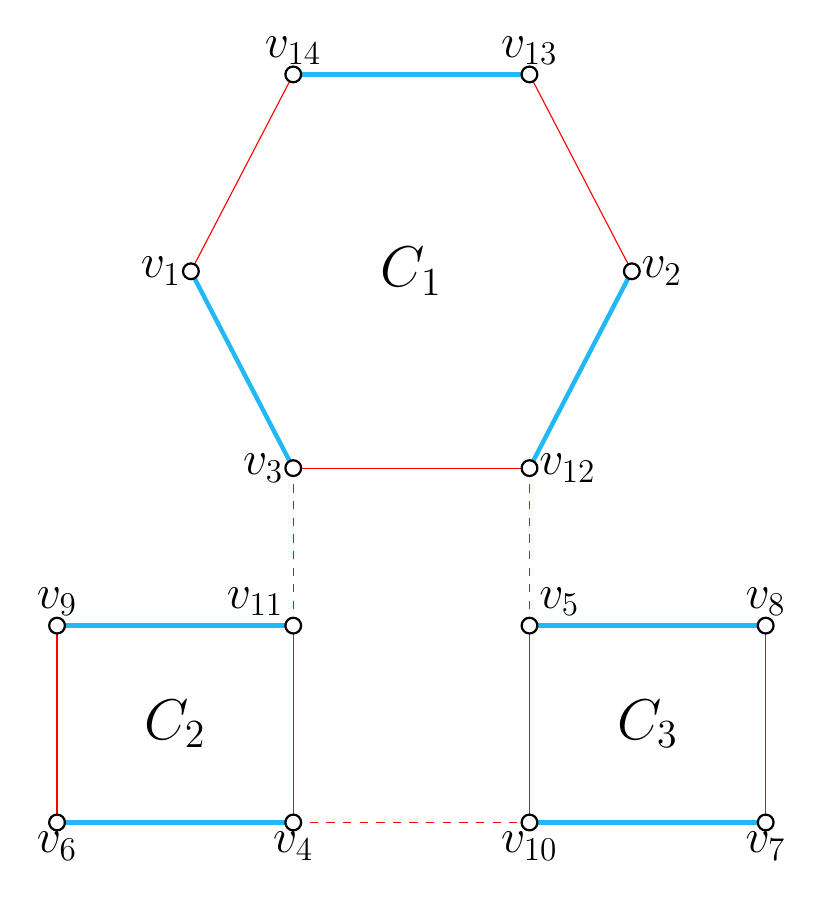
\begin{tikzpicture}
%\draw [help lines] (-1,-1) grid (12, 12);

%C1 - blue
\draw [ultra thick, myBlue] (3,9.5) -- (6,9.5); %v14 - v13
\draw [ultra thick, myBlue] (3,4.5) -- (1.7,7); %v3 - v1
\draw [ultra thick, myBlue] (6,4.5) -- (7.3,7); %v12 - v2

%C2 - blue
\draw [ultra thick, myBlue] (0,0) -- (3,0); %v6 - v4
\draw [ultra thick, myBlue] (0,2.5) -- (3,2.5); %v9 - v11

%C3 - blue
\draw [ultra thick, myBlue] (6,0) -- (9,0); %v10 - v7
\draw [ultra thick, myBlue] (6,2.5) -- (9,2.5); %v5 - v8

%C1 - red
\draw [myRed] (3,4.5) -- (6,4.5); %v3 - v12
\draw [myRed] (1.7,7) -- (3,9.5); %v1 - v14
\draw [myRed] (7.3,7) -- (6,9.5); %v2 - v13

%C2 - red
\draw [myRed] (0,0) -- (0,2.5); %v6 - v9
\draw [myRed] (3,0) -- (3,2.5); %v4 - v11

%C3 - red
\draw [myRed] (6,0) -- (6,2.5); %v10 - v5
\draw [myRed] (9,0) -- (9,2.5); %v7 - v8

%Connecting edges
\draw [dashed, myRed] (3,2.5) -- (3,4.5); %v11 - v3
\draw [dashed, myRed] (6,2.5) -- (6,4.5); %v5 - v12
\draw [dashed, myRed] (3,0) -- (6,0); %v4 - v10 


%C1 - vertices
\draw [fill=white, thick] (3,4.5) circle [radius = 0.1]; %v3
\draw [fill=white, thick] (6,4.5) circle [radius = 0.1]; %v12
\draw [fill=white, thick] (1.7,7) circle [radius = 0.1]; %v1
\draw [fill=white, thick] (7.3,7) circle [radius = 0.1]; %v2
\draw [fill=white, thick] (3,9.5) circle [radius = 0.1]; %v14
\draw [fill=white, thick] (6,9.5) circle [radius = 0.1]; %v13

%C2 - vertices
\draw [fill=white, thick] (0,0) circle [radius = 0.1]; %v6
\draw [fill=white, thick] (3,0) circle [radius = 0.1]; %v4
\draw [fill=white, thick] (0,2.5) circle [radius = 0.1]; %v9
\draw [fill=white, thick] (3,2.5) circle [radius = 0.1]; %v11

%C3 - vertices
\draw [fill=white, thick] (6,0) circle [radius = 0.1]; %v10
\draw [fill=white, thick] (9,0) circle [radius = 0.1]; %v7
\draw [fill=white, thick] (6,2.5) circle [radius = 0.1]; %v5
\draw [fill=white, thick] (9,2.5) circle [radius = 0.1]; %v8


%C1 - labels
\node [left] at (3,4.5) {\LARGE{$v_3$}};
\node [right] at (6,4.5) {\LARGE{$v_{12}$}};
\node [left] at (1.7,7) {\LARGE{$v_1$}};
\node [right] at (7.3,7) {\LARGE{$v_2$}};
\node [above] at (3,9.5) {\LARGE{$v_{14}$}};
\node [above] at (6,9.5) {\LARGE{$v_{13}$}};

%C2 - labels
\node [below] at (0,0) {\LARGE{$v_6$}};
\node [below] at (3,0) {\LARGE{$v_4$}};
\node [above] at (0,2.5) {\LARGE{$v_9$}};
\node [above left] at (3,2.5) {\LARGE{$v_{11}$}};

%C3 - labels
\node [below] at (6,0) {\LARGE{$v_{10}$}};
\node [below] at (9,0) {\LARGE{$v_7$}};
\node [above right] at (6,2.5) {\LARGE{$v_5$}};
\node [above] at (9,2.5) {\LARGE{$v_8$}};

%Component labels
\node at (4.5,7) {\huge{$C_1$}};
\node at (1.5,1.25) {\huge{$C_2$}};
\node at (7.5,1.25) {\huge{$C_3$}};


\end{tikzpicture}
	
\end{document}
